\documentclass[fleqn]{homework}

\student{Stephen Brennan (smb196)}
\course{EECS 440}
\assignment{Programming 1}
\duedate{September 24, 2015}

%\usepackage{mathtools}
%\usepackage{graphicx}

\begin{document}
  \maketitle

  In this assignment, I implemented a decision tree learning algorithm.  For the
  most part, the implementation was straightforward, although a major concern
  was the runtime of the cutoff selection for continuous attributes.  My
  implementations run rather slowly, but I was able to get complete data by
  running many processes on my research computing server.

  It would be very useful if in the future, the code template was designed such
  that we could produce accuracy vs depth data by training partially,
  predicting, and then training further, and then predicting again.  This would
  be much more efficient, since when we run the code multiple times at different
  depths, we waste time retraining the smaller depths of the tree before getting
  to the larger depths.

  \begin{problem}{a}
    \begin{question}
      What is the accuracy of the classifier on each dataset when the depth is
      set to 1? (i.e. the tree has just 1 test)
    \end{question}
    To answer this question, I set the depth to be 2, because my implementation
    includes the leaf nodes in the accounting of depth.

    \begin{tabular}{lll}
      \textbf{Dataset} & \textbf{Accuracy} & \textbf{Majority Prop.} \\
      \hline
      \textit{Voting} & 0.984 & 0.555 \\
      \textit{Volcanoes} & 0.674 & 0.672 \\
      \textit{Spam} & 0.643 & 0.625 \\
    \end{tabular}

    I've provided the accuracy at depth 2 along with the majority class label,
    since the baseline for accuracy comparison should be the accuracy you would
    get by predicting the majority class label, which is simply the proportion
    of examples which have the majority class label.  By showing this on the
    same chart, you can see that \textit{voting} was by far the most successful
    with just a single test, and that although \textit{spam} had a lower
    accuracy than \textit{volcanoes} with a single test, it represented a much
    more meaningful improvement from the baseline than \textit{volcanoes} had.
  \end{problem}

  \begin{problem}{b}
    \begin{question}
      For \textit{spam} and \textit{voting}, look at first test picked by your
      tree. Do you think this intuitively looks like a sensible test to perform
      for these problems?  Explain.
    \end{question}

    For \textit{voting}, the first test picked by my tree was attribute 0.  This
    was a bill about repealing the Affordable Health Care Act, which is a
    \textit{quite} polarizing issue.  It makes complete sense that this was the
    most predictive attribute, given the highly partisan nature of the bill.

    For \textit{spam}, the first test picked by my tree was ``is the
    geographical distance less than 2.69''.  If true, it would predict negative
    (not spam).  If false, it would predict positive (spam).  This makes a lot
    of sense, given that a person is probably more likely to want mail from
    somebody close to them, and spam is more likely sent from a central place
    that is far away from most of its recipients.  This strategy alone results
    in 64.3\% accuracy in 5-fold validation, if you limit to a depth of two.
  \end{problem}

  \begin{problem}{c}
    \begin{question}
      For \textit{volcanoes} and \textit{spam}, plot the accuracy as the depth
      of the tree is increased. On the x-axis, choose depth values to test so
      there are at least five evenly spaced points. Does the accuracy improve
      smoothly as the depth of the tree increases? Can you explain the pattern
      of the graph?
    \end{question}
    
    Plots are presented below.  I found that \textit{volcanoes} had very bad
    overall accuracy: it did not improve beyond the proportion of majority class
    labels.  The variance that can be seen in the plot is likely explained due
    to the variability in the sampling in the $k$ fold validation.  On the other
    hand, \textit{spam} shows mild improvement as the depth increases at first,
    but doesn't increase much beyond a small depth.  I would expect that this is
    because some of the attributes provide duplicate information, and also that
    the decision tree quickly reaches the limit of the decision surface it can
    represent.

    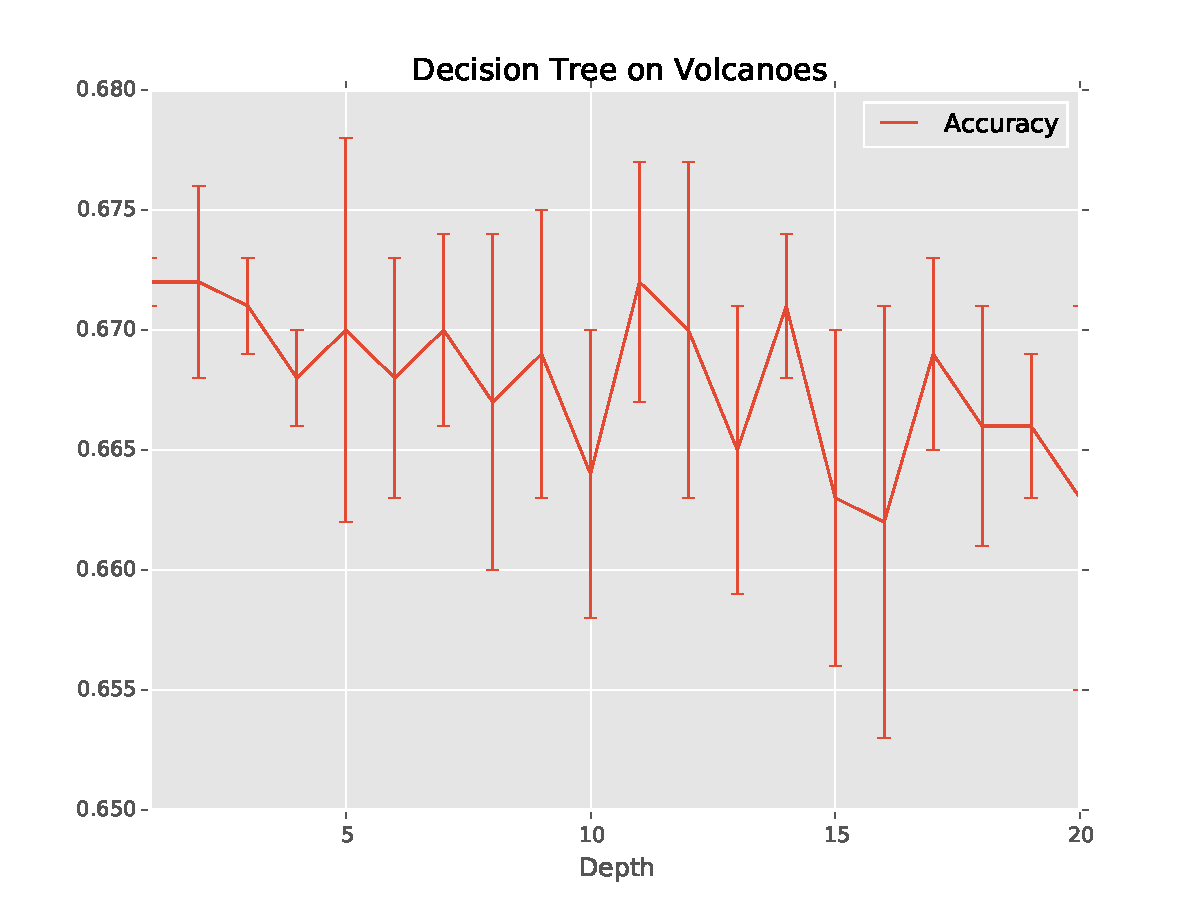
\includegraphics[width=0.48\textheight]{volcanoes.pdf}

    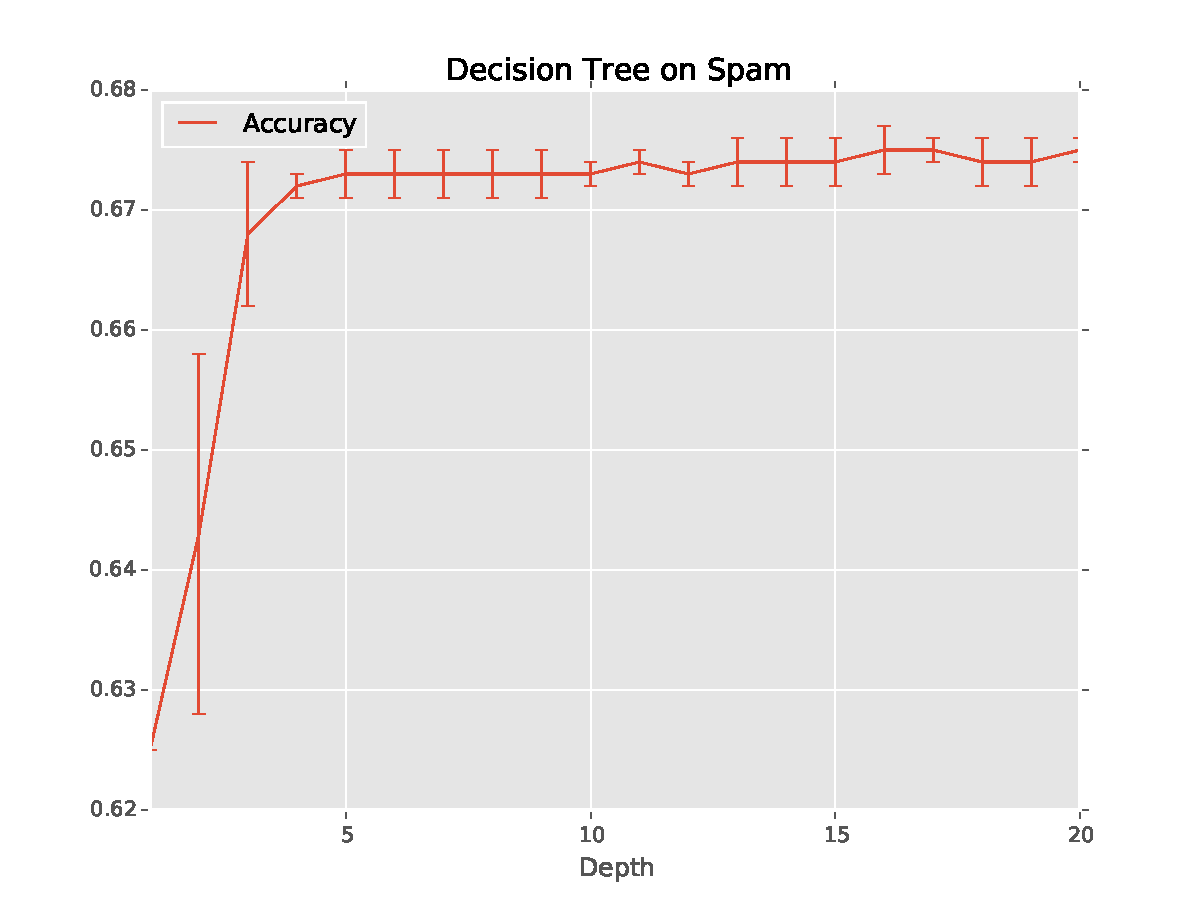
\includegraphics[width=0.48\textheight]{spam.pdf}
  \end{problem}

\end{document}